
\chapter{Modelo macroscópico para la dinámica de población de las células T durante la respuesta inmune.}
\label{cap:modeloMacroscopico}

En este capítulo se expone otro modelo matemático propuesto para determinar el algoritmo de decisión entre división o apoptosis de las células T durante una respuesta inmune (ver Sección \ref{cuestionAmodelizar}). En esta área aún son muchas las cuestiones que quedan por resolver: una vez que las células se activan, ¿hasta cuándo continúan dividiéndose?, ¿es esta decisión totalmente dependiente de las condiciones que hayan tenido las células en el momento de su activación?, ¿por qué hay un retraso respecto a la desaparición del \textit{patógeno} en la \textit{contracción clonal}?... Estas cuestiones se atajaron en el Capítulo \ref{cap:descripcionTrabajo}, donde se establece la base teórica de un modelo matemático a nivel microscópico. Es decir, este modelo proporciona el algoritmo de decisión para cada célula, pues las decisiones de las células inmunes son, \textit{a priori}, independientes unas de otras (no se ha encontrado un órgano que regule estos mecanismos \citep{arias2016emergent}).

En este capítulo lo que haremos será volver sobre este mismo problema, pero desde una perspectiva un poco distinta, desde un punto de vista macroscópico. Esto quiere decir que las ecuaciones diferenciales sobre las que se basa el modelo determinan el comportamiento de toda la población de células. Para entender esto podemos poner como ejemplo los movimientos de un equipo de fútbol: la estrategia de contraataque del equipo vista desde el punto de vista <<macroscópico>> sería recuperar el balón y avanzar rápidamente al campo del adversario para marcar gol. Sin embargo, si nos fijamos ahora en el mundo <<microscópico>> de cada jugador, vemos que cada uno tiene su papel, defender y recuperar la posesión, pasar a los centrales o a los delanteros, etc.

%Al comienzo de este capítulo, en la Sección \ref{sec:toler_tasaCrecim}, se aborda la relación entre el caso de tolerancia al \textit{patógeno} y la tasa de crecimiento de este. Por su parte la Sección \ref{sec:iner_elast} desgrana las dos características poblacionales, incercia y la elasticidad, sobre las que se sustenta el modelo. En la última sección (Sección \ref{sec:simu_macro}), se realizan simulaciones de este modelo y se comparan los resultados con los del modelo microscópico.

Al comienzo de este capítulo, la Sección \ref{sec:iner_elast} desgrana las dos características poblacionales, incercia y la elasticidad, sobre las que se sustenta el modelo y se detallan las ecuaciones que rigen la dinámica de población de las células T y del \textit{patógeno}. En la sección siguiente (Sección \ref{sec:simu_macro}), se realizan simulaciones de este modelo y se comparan los resultados con los del modelo microscópico.


%\section{Tolerancia y tasa de crecimiento}
%\label{sec:toler_tasaCrecim}

%La respuesta inmune adaptativa se basa en la capacidad que tienen las células T para identificar diferentes \textit{antígenos} pero ¿cómo saber cuáles de ellos son amigos y cuáles enemigos? En esta sección asumiremos que las células T toleran células cuyas tasas de crecimiento permanezcan por debajo de cierto límite, es decir, aquellas que no crezcan con mucha rapidez (las células que crecen muy rápidamente se asocian con toxinas o células tumorales, por ejemplo \citep{arias2015growth}). Además, nos centraremos en dos características de la dinámica de población de las células T: la elasticidad (la población se expande y se contrae, lo conocemos como \textit{expansión} y \textit{contracción clonal}) y la inercia (la \textit{contracción clonal} se presenta con retraso tras la desaparición del \textit{patógeno}) \citep{arias2015growth}. Este resultado permite dar una posible explicación al hecho paradójico de que aquellos \textit{patógenos} que se reproducen más lentamente en un organismo sean tolerados por las células inmunes.


\section{Inercia y elasticidad en las células T}
\label{sec:iner_elast}


Como ya se avanzaba en la introducción de este capítulo, nos centraremos en dos características de la dinámica de población de las células T: la elasticidad (la población se expande y se contrae, lo conocemos como \textit{expansión} y \textit{contracción clonal}) y la inercia (la \textit{contracción clonal} se presenta con retraso tras la desaparición del \textit{patógeno}) \citep{arias2015growth}. En base a estas dos propiedades, se detallan las ecuaciones que dan lugar a este modelo matemático. El modelo consta de un sistema de ecuaciones diferenciales de segundo orden. Este tipo de ecuaciones constituye la manera más simple de representar la inercia de la población \citep{arias2015growth}. Además, las ecuaciones de segundo grado son el marco general para las dinámicas \textit{newtonianas}. Esto nos lleva a modelar de manera natural la dinámica de las células T efectoras como el balance entre dos fuerzas opuestas actuando sobre la población: una fuerza por parte del \textit{antígeno} causada por la presencia del \textit{patógeno} y una fuerza intrínseca elástica que devuelve a la población a su estado inicial. En concreto, asumiremos que la fuerza que ejerce el \textit{antígeno} es proporcional al número de células del \textit{patógeno} y modelaremos la elasticidad mediante la \textit{Ley de Hooke}, que establece que la fuerza necesaria para restablecer el equilibrio una vez que la población ha llegado a cierto valor es proporcional a dicho valor \citep{arias2015growth}. También asumiremos que el \textit{patógeno} prolifera con una ratio constante y que serán eliminados por la acción de las células T de manera proporcional a sus encuentros mutuos. De esta manera, presentamos el siguiente modelo:

\begin{equation}
	\label{sist_macro}
	\left\{ \begin{array}{l}
	{T^{\prime\prime}}(t) = -kT(t) + \lambda P(t) \\
	{P^{\prime}}(t) = \alpha P(t) - \beta T(t)P(t) \\
	\\
	T(0)=0 \hspace{3cm} ,para\, T \geq 0,\, P \geq P_m \\
	T^{\prime}(0)=0  \\
	P(0)=P_0 \geq P_m  \\ 
	\end{array}
	\right.
\end{equation}

Donde $T(t)$ y $P(t)$ son el número de células T efectoras y el número de células de \textit{patógeno}, respectivamente. La primera ecuación diferencial que nos encontramos nos sugiere que, en ausencia de \textit{patógeno}, la población de células T se puede caracterizar por una respuesta elástica en forma de soluciones oscilatorias. Así mismo, la presencia de \textit{patógeno} tendría el efecto de una fuerza externa. Siguiendo con la segunda ecuación, observamos que, en ausencia de células T, la población de \textit{patógeno} crece de manera exponencial. Sin embargo, una vez que las células T entran en acción empiezan a eliminar al \textit{patógeno} de acuerdo a posibles encuentros entre $T(t)$ y $P(t)$ \citep{arias2016emergent}. La eficiencia de cada proceso se mide en base a cuatro parámetros y las condiciones iniciales del sistema. Estos parámetros son $\alpha$, $\beta$, $k$ y $\lambda$. Los dos primeros representan la tasa de crecimiento del \textit{patógeno} y la tasa de eliminación del mismo a causa de las células T, respectivamente. Por su parte $k$ y $\lambda$ representan las constantes de elasticidad e inercia de la población, respectivamente. Una diferencia entre este modelo y otras teorías propuestas para el caso de la tolerancia inmune es que la percepción de la ratio de crecimiento del \textit{antígeno} viene determinado como una propiedad general a toda la población. Mientras la decisión de activación puede ser tomada por células T en estado \textit{naïve} en base a la información local sobre las \textit{células presentadoras de antígeno}, el momento en el que comienza la \textit{contacción clonal} no puede ser establecido por ninguna célula T. Cada célula T tiene una información muy limitada acerca de la progresión de una respuesta inmune y es improbable que una célula T pueda medir, de manera individual, la ratio de crecimiento de las células que presentan ese mismo \textit{antígeno}. Sin embargo, propiedades colectivas como la inercia o la elasticidad pueden permitir a la población de células T distinguir entre una respuesta aguda o la tolerancia al \textit{patógeno} \citep{arias2015growth}.

El Sistema \ref{sist_macro} también puede expresarse de manera adimensional, reduciendo el número de parámetros a dos: 

\begin{equation}
	\label{sist_macro_nod}
	\left\{ \begin{array}{l}
	{T^{\prime\prime}}(t) = -T(t) + P(t) \\
	{P^{\prime}}(t) = \alpha^{*} P(t) - \beta^{*} T(t)P(t) \\
	\\
	T(0)=0 \hspace{3cm} ,para\, T \geq 0,\, P \geq P_m^{*} \\
	T^{\prime}(0)=0  \\
	P(0)=1 \\ 
	\end{array}
	\right.
\end{equation}

Donde $\alpha^{*} = \frac{\alpha}{\sqrt k}$, $\beta^{*} = \frac{\beta \lambda P_0}{k \sqrt k}$ y $P_{m}^{*} = \frac{P_m}{P_0}$.

En lo que sigue veremos el comportamiento de estos dos sistemas mediante una serie de simulaciones numéricas, pues en este caso las ecuaciones no tienen una solución explícita.

\section{Simulaciones del modelo macroscópico}
\label{sec:simu_macro}

A continuación, presentaremos distintas situaciones que se pueden dar con la simple variación de los parámetros del modelo macroscópico visto en la sección anterior. Para poder comparar estos resultados, se simulan las situaciones de tolerancia e intolerancia vistas en el Capítulo \ref{cap:simulaciones} para el modelo microscópico y veremos cómo los parámetros $\alpha^{*}$ y $\beta^{*}$ del Sistema \ref{sist_macro_nod} nos revelan la dependencia crucial que tienen sobre el modelo en estas dos situaciones.

El código referente a esa sección puede verse en el Apéndice \ref{Appendix:A}.



\subsection{Intolerancia al \textit{patógeno}}
\label{sub:simMacroIntoler}

Como vimos en la Sección \ref{sim:intoler}, el caso de intolerancia al \textit{patógeno} se da cuando las células inmunes consiguen eliminar al agente que causa la infección. 
En este tipo de simulaciones vemos como el \textit{patógeno} aumenta su población seguido de una rápida proliferación de las células T (\textit{expansión clonal}), cuya acción erradica al \textit{patógeno}. Posteriormente a la desaparición del \textit{patógeno}, y con cierto retraso, tiene lugar la \textit{contracción clonal}, que restaura los niveles de población de células T. En la Figura \ref{fig:macro_intolerance}, correspondiente a a simulación del Sistema \ref{sist_macro}, podemos ver esta situación gráficamente. 

Queda, por tanto, de manifiesto la característica de inercia, pues se ve cómo las células T comienzan a disminuir en número tiempo después de que el \textit{patógeno} haya desaparecido, y de elasticidad, pues la población de células T acaba recuperando sus niveles iniciales. Como vemos, el parecido de esta figura con la Figura \ref{fig:intolerance} es notable, ambos modelos, macroscópico y microscópico, simulan el mismo comportamiento desde dos puntos de vista distintos.


\begin{figure}[t]
	\centering
	\begin{tabular}{cc}
		\subfloat [Simulación: caso de intolerancia al \textit{patógeno} en el modelo macroscópico. Parámetros: $\alpha=1,5$, $\beta=0,1$, $k=4$, $\lambda=0.5$, $P_m = 0$.]{
			\label{fig:macro_intolerance}
			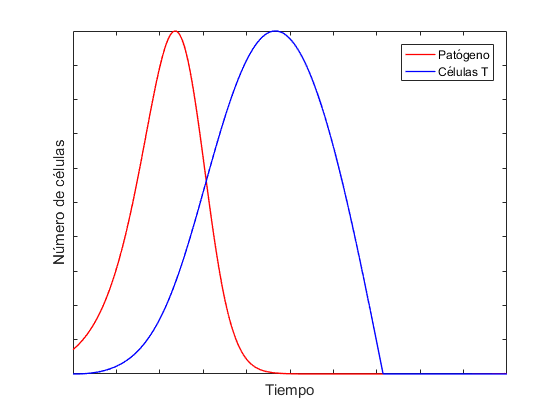
\includegraphics[width=0.5\textwidth]{Imagenes/Simulaciones/macro_intoler}}
		& \subfloat[Simulación: caso de tolerancia al \textit{patógeno} en el modelo macroscópico. Parámetros: $\alpha^{*}=1,1$, $\beta^{*}=0,01$, $P_m^{*} = 0$.]{
			\label{fig:macro_tolerance}
			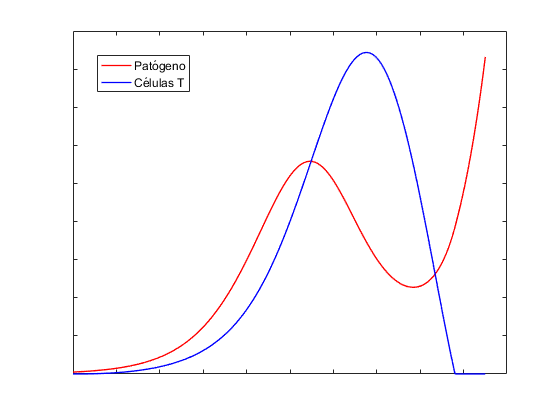
\includegraphics[width=0.5\textwidth]{Imagenes/Simulaciones/macro_toler}}\\
	\end{tabular}
	\caption{Simulaciones del modelo macroscópico. Casos de intolerancia y tolerancia al \textit{patógeno}}%\label{foo}
\end{figure}

\subsection{Tolerancia al patógeno}
\label{sub:simMacroToler}

Veamos ahora al caso análogo a la Sección \ref{sim:toler}, donde vimos cómo un \textit{patógeno} con una tasa de reproducción pequeña conseguía zafarse de las células T. En la Figura \ref{fig:macro_tolerance} puede observarse que las células T comienzan la \textit{contracción clonal}, haciendo que su población desaparezca irremediablemente, y provocando que el \textit{patógeno} pueda reproducirse sin ningún tipo de impedimento, ya que no desaparece, simplemente se reproduce más lento. En este caso la simulación corresponde al Sistema \ref{sist_macro_nod}.

%\begin{figure}[t]
%	\centering
%	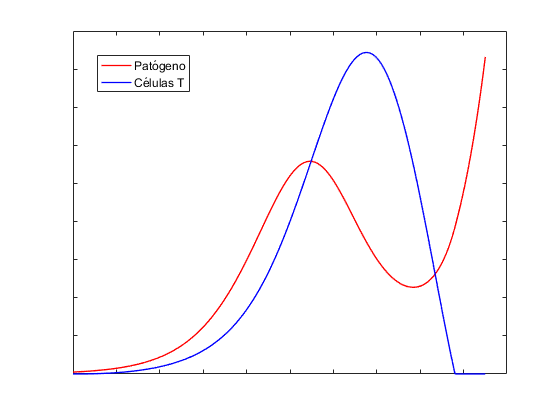
\includegraphics[width=0.7\textwidth]{Imagenes/Simulaciones/macro_toler}
%	\caption{Simulación: caso de tolerancia al \textit{patógeno} en el modelo macroscópico.\\Parámetros: $\alpha^{*}=1,1$, $\beta^{*}=0,01$.}
%	\label{fig:macro_tolerance}
%\end{figure}



\subsection{Regiones de tolerancia e intolerancia}
\label{sub:reg_tolerIntolerMacro}

Un análisis interesante que se puede hacer es determinar qué relación existe entre el valor de los parámetros del modelo y las regiones de intolerancia y tolerancia. Este asunto se ha abordado para el modelo macroscópico adimensional (ver Sistema \ref{sist_macro_nod}). Para ello se ha implementado un programa que recorre los valores de $\alpha^{*}$ y $\beta^{*}$ entre $0,1$ y $2,5$ con un paso de $0,1$\footnote{Con paso nos referimos al valor del incremento del parámetro en cada iteración.}, y, para cada valor, simula el Sistema \ref{sist_macro_nod}. Una vez hecha la simulación se observa el número de células T y de \textit{patógeno} para obtener el resultado de tolerancia, en caso de que las células T no consiguen acabar con el \textit{patógeno} o intolerancia en caso contrario. La Figura \ref{fig:macro_toler_intoler} recoge el resultado de todas estas simulaciones, arrojando datos importantes: si dejamos uno de los dos parámetros fijos, es posible cambiar de una región a otra con tan solo modificar el otro parámetro. De hecho, de acuerdo con este modelo, \textit{patógenos} y tumores pueden escapar de la acción de las células T por dos métodos: reduciendo el efecto de las células T, el parámetro $\beta^{*}$, o reduciendo su tasa de proliferación, el parámetro $\alpha^{*}$, \citep{arias2016emergent}. Una consecuencia que se puede extraer de esto es que mecanismos como la fiebre, que incrementa la tasa de proliferación del \textit{patógeno}, o la inflamación, que aumenta la acción de las células T, favorecen que el \textit{patógeno} sea vencido. 

\begin{figure}[t]
	\centering
	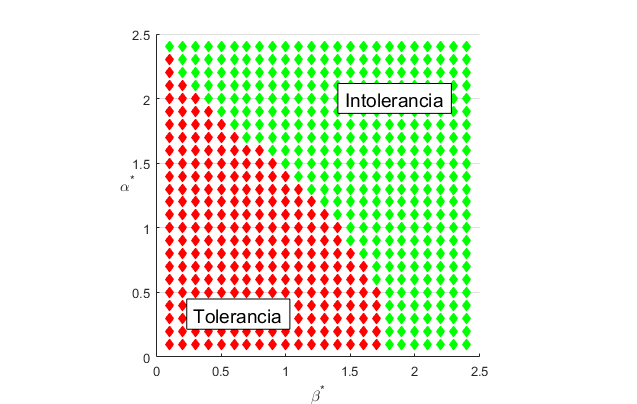
\includegraphics[width=1\textwidth]{Imagenes/Simulaciones/macro_toler_intoler}
	\caption{Simulación del modelo macroscópico adimensional. Variación de los parámetros $\alpha^{*}$ y $\beta^{*}$ para dar lugar a regiones de tolerancia e intolerancia al \textit{patógeno}.}
	\label{fig:macro_toler_intoler}
\end{figure}